\documentclass[letterpaper]{aamas2015}
%\usepackage{times}
%\usepackage{helvet}
%\usepackage{courier}
\usepackage{mathptmx}
\usepackage{graphicx}
\usepackage{amsmath}
\usepackage{microtype}
\usepackage{wrapfig}
\usepackage{color}
\usepackage{latexsym}
\usepackage{amssymb}
\usepackage{multirow}
\usepackage{seanmacros}
\usepackage{xfrac}
%\usepackage{fixbib}

%\frenchspacing
\setlength{\pdfpagewidth}{8.5in}
\setlength{\pdfpageheight}{11in}
%\pdfinfo{
%/Title Bounty Hunters and Multiagent Task Allocation
%/Author Drew Wicke, David Freelan, Sean Luke   
%/Keywords MAS: Ad-hoc teamwork, MAS: Multiagent Learning, MAS: Multiagent Systems (General/other), GTEP: Auctions and %Market-Based Systems
%}
\setcounter{secnumdepth}{0}  

%%% AAMAS requires a period after paragraph headers.  But we have a
%%% header ending in a ?.  We fix this by modifying the class file so the
%%% period does not automatically appear, and then create a special command
%%% below for the more common case.
\newcommand\paragrapha[1]{\paragraph*{{#1}.}}

\newcommand\citenauthor[1]{\citen{#1}}
\newcommand\citenyear[1]{\citen{#1}}
\sloppy

\newcommand\citen[1]{\hbox{\cite{#1}}}
\newcommand{\goodhline}{\vspace{-1em}\\\hline\vspace{-0.9em}\\}
%\newcommand{\gooditem}{\vspace{0.2em}\item}
\newcommand{\gooditem}{\item}

%\newcommand\hitab{{\footnotesize\textsf{HiTAB}}}
%\newcommand\hitabbig{{\normalsize\textsf{HiTAB}}}

\newcommand\hitab{HiTAB}
\newcommand\hitabbig{HiTAB}

\newcommand\bump{\vspace{10in}}
\DeclareMathOperator*{\argmax}{argmax}

\begin{document}

\title{Adaptive Bondsman and Efficient Multiagent Task Allocation}

%\author{Drew Wicke \qquad David Freelan \qquad Sean Luke\\
%Department of Computer Science, George Mason University\\
%4400 University Drive MSN 4A5\\
%Fairfax VA 22314 USA\\
%}
\numberofauthors{1}

\author{
% You can go ahead and credit any number of authors here,
% e.g. one 'row of three' or two rows (consisting of one row of three
% and a second row of one, two or three).
%
% The command \alignauthor (no curly braces needed) should
% precede each author name, affiliation/snail-mail address and
% e-mail address. Additionally, tag each line of
% affiliation/address with \affaddr, and tag the
% e-mail address with \email.
% 1st. author
\alignauthor
%Paper XXX
Drew Wicke\\
       \affaddr{Department of Computer Science}\\
       \affaddr{George Mason University}\\
       \affaddr{4400 University Drive MSN 4A5}\\
       \affaddr{Fairfax, VA 22030, USA}\\
       \email{dwicke@gmu.edu}
       }


\maketitle

\begin{abstract}

We explore the bondsman in a system for multiagent task allocation inspired by the model used by bounty hunters and bail bondsmen.  A bondsman posts tasks for agents to complete, along with bounties to be collected by an agent on completion.  Multiple agents, taking the role of the bounty hunters, compete to finish tasks and collect their bounties.  While a task remains uncompleted, its bounty gradually rises, making it more and more desirable to pursue.  Unlike auctions, this model does not assume rationality in agents' bids (as there are none), and since tasks are not exclusive to given agents, the system is robust to highly noisy environments.  We examine how the bondsman can adaptively adjust exclusivity of tasks and the reward function in order to minimize redundant agents.  We also look at the corresponding problem of improving the bounty hunter's learning algorithm to better handle dynamically changing exclusivity of the tasks. We compare different approaches to adaptive bondsman, and we do so under both static environments and ones in which agents, and task details, change dynamically and we compare against the results from our original research.  

\end{abstract}

\category{I.2.11}{Distributed Artificial Intelligence}{Multiagent Systems}

%A category including the fourth, optional field follows...
%\category{D.2.8}{Software Engineering}{Metrics}[complexity measures, performance measures]

%General terms should be selected from the following 16 terms: Algorithms, Management, Measurement, Documentation, Performance, Design, Economics, Reliability, Experimentation, Security, Human Factors, Standardization, Languages, Theory, Legal Aspects, Verification.

\terms{Algorithms, Experimentation, Performance}

%Keywords are your own choice of terms you would like the paper to be indexed by.

\keywords{Bounty Hunting; Auctions; Task Allocation}




\section{Introduction} 

The {\it dynamic multiagent task allocation problem} is one in which one or more agents collectively perform tasks as they appear dynamically in the environment.  The agents typically vary in their ability to perform various tasks, and as this is a {\it multiagent} problem, there is no one agent who decides how to allocate the tasks to them.  Rather, the agents decide on their own what tasks they should vie for, with certain limitations on the degree to which they may consult one another to make these decisions.   Ideally, out of a morass of individual greedy agent decisions, we would see a task allocation which approaches optimal global efficiency.

Scenarios such as these crop up throughout multiagent systems: they appear in robots divvying up room cleaning needs; or automated multiagent delivery services; or video games where a band of plucky outlaws must defend themselves against hordes of zombies.  Considerable study over the years has focused on centralized approaches to globally optimal dynamic task allocation, involving areas such as register coloring and pebbling, multi-armed bandits, and bin packing.  When the problem is restricted to the multiagent case, most work has focused on greedy methods, the most popular approach being  {\it auctions}.

A simple auction method might work as follows.  There is a single auctioneer who distributes tasks, and multiple agents who bid on the privilege to do them.  As tasks come available, agents compete with bids in an auction, and after a clearing time has passed, the winning agent is given the task to complete.  Typically the agents will bid their {\it valuation} of the task, that is, some estimate the agent has of how good the task would be for the agent to do.

This approach is intuitive and appealing at first glance, but it has some curiosities.  First, in much of the literature, there is no incentive or reward for agents to complete a task.  Second, agents generally have an infinite money supply, and so we must presume they are altruistic and non-strategic.  Third, winning agents usually have exclusive ownership of tasks, so some other mechanism (perhaps real options) must be implemented to deal with agents with poor or noisy task performance.  Fourth, agents typically must have some built-in ability to produce an accurate valuation of the tasks they are bidding on.    Fifth,  auction methods commonly assume that tasks are bid on sequentially as they arrive, perhaps necessitating a multi-task mechanism for each agent or a clearing time.  For these reasons and others, auctions seem to us to be an odd approach to task allocation.  
%In the real world, people do not bid on the privilege to do work: at the very least, they might bid on the option or contract to do work in return for some payment.

In this paper we study an alternative model which seems to us to be a closer fit to the dynamic multiagent task allocation problem: {\it bounty hunting.}  Here, the auctioneer is replaced with a bail bondsman, and the agents are no longer bidders, but bounty hunters.

A quick explanation of these terms for those who may be unfamiliar with them.  In the United States, an arrested man may be set free temporarily prior to his trial in return for some amount of money ({\it bail}) as collateral.   Bail is often costly, so there is an industry of {\it bail bondsmen} who will, for a fee, post bail on behalf of the arrested man.  If the man does not show for his trial, a bail bondsman can recover his posted bail only if he brings the fugitive back to be tried before the government has re-arrested him.  To do this, the bail bondsman will offer some amount of reward (a {\it bounty}) to anyone who successfully captures the fugitive.   The competing agents who try to capture the fugitive in return for this bounty are {\it bounty hunters}.  While the fugitive is still at large, the bounty may be increased so as to make his capture more lucrative.   This model appears elsewhere in different guises of course: for example, a reward for a lost cat, a Most Wanted Criminal list, a murder contract, or a software bug bounty. 

Bounties are an attractive approach to the dynamic multiagent task allocation problem for several reasons.  First, because agents may compete for the same bounty, tasks are no longer exclusive.  If an agent cannot successfully do a given task, eventually its bounty will rise and attract other agents to take it from him.  Second, there is no bidding involved: agents can be self-interested, though still perhaps not hyperstrategic, and there is no need for a queue or clearing interval.  Finally, since agents are not bidding their valuation, they don't need to have (at least initially) an accurate valuation mechanism in the first place.

But despite their seemingly natural fit, bounties have surprisingly been little studied in multiagent systems.  We were the first to apply bounty hunting to the dynamic multiagent task allocation problem in DREW ADD AAMAS PAPER!!!.  In this paper we will continue the study of bounty hunting, but instead focusing on the bondsman.  We first describe the formal bounty system and then we define the adjustments to the bondsman and the bounty hunter we made.  In all these approaches agents have no initial valuation of tasks, so we then examine how they may adapt to develop a proper valuation, and thus improve global system performance.  We will also examine how well this adaptation performs when the nature of tasks, or the agents, changes radically.

\section{Related Work}

A taxonomy of solutions to the general multiagent task allocation problem has been offered~\cite{Gerkey:2004} with three major dimensions: the type of task, the type of agent, and the information available to determine task assignment.  This taxonomy has recently been improved to classify more task allocation problems, like those where tasks have dependencies \citen{Korsah:2013}.  Current solution methods include centralized approaches using k-armed bandits, integer programming, and combinatorial optimization; and decentralized approaches like auctions, markets, and task swapping \citen{Lagoudakis:2004,Liu:2014,Liu:2012,Nanjanath:2006}.


We are primarily interested in the decentralized case.  The most common approach, auctions, were popularized by MURDOCH, an auction method which focused on minimizing resource usage, task completion time, and communication overhead \citen{Gerkey2002c}.  
%MURDOCH was work is based off of the contract net protocol \citen{Smith:1980}.
This approach trusted agents to truthfully bid their task valuations, though sensor noise or an unknown environment could cause their bids to be inaccurate.  TraderBots, another auction framework, was designed to be more flexible and extensible \citen{Dias:2004,Jones:2006}.  Auctions have been augmented to be robust to robot malfunctions \citen{Nanjanath:2010}.  CoMutaR merged  multiagent task allocation with coordination through the use of auctions under the assumption of truthful agents \citen{Shiroma:2009}.  We are aware of only one paper that has considered approaches to extend auctions with non-exclusivity and non-commitment~\cite{Mataric:2003}.

Markets have also been used in multi-robot task allocation \citen{Botelho:1999,Pustowka:2012} and exploration \citen{Simmons:2000,Zlot:2002}.   One paper describes a market based planning system in which the agents learn to bid their opportunity cost for doing a task, and tasks have rewards associated with them, allowing agents to re-auction them \citenauthor{Schneider:2005}.

Another approach is {\it token-passing} \citen{Farinelli:2005}.  This method, like auctions and markets, also assumes task exclusivity.  But like some market methods, it allows the tasks to be reassigned by passing the token to other agents.  Similarly,  \citenauthor{Dahl2003} used {\it vacancy chains} as a method for allocating tasks.  A vacancy chain is a social construct where when one agent receives a task, he releases his previous task, which goes to another agent in the chain, who releases his task, and so on.  Finally, L-ALLIANCE adapted threshold parameters determining how robots choose tasks \citen{Parker1995,Parker1998}.  


A few auction methods have agents that use adaptive mechanisms for bidding.  For example, \cite{Jones:2007} use Support Vector Regression to formulate a bid for a task in domains where some tasks can't be completed due to a lack of resources.  Another adaptive bidding procedure for task allocation was developed in \cite{Choi:2013} and was used to bid in a sequential auction with a clearing time.  In a method developed by \cite{Pippin:2013}, the auctioneer, rather than the bidders, is adaptive and weights the bids for tasks based on each agent's success rate.  This is very close to a centralized approach.  One non-auction task allocation method \cite{Campbell:2008} uses biologically inspired adaptive agents that have an upper and lower bound for going after tasks with particular difficulties (similar to L-ALLIANCE), where the lower threshold changes based on task difficulty distribution. Because of the strong assumptions these adaptive auctions make, they could be adapted to our target problem case only with radical modification.  We have instead taken a different approach for comparison: adapting our proposed bounty mechanism into one which has certain the basic features (notably exclusivity) of an auction.  


Bounties are a subset of {\it contests}, scenarios where agents are pit against one another to obtain a prize \cite{Corchon:2007}.  One type of contest, the {\it tournament}, is very common in sports and competitions \cite{Connelly:2014}, and contests are also found throughout economics, and in the managerial and political sciences \cite{Konrad:2009}.  Contests have not been applied much in multiagent task allocation to date. Contest theory has explored adjustable incentive mechanisms in terms of promotions within companies and cash prizes based on performance \cite{Casas:2009,Nalebuff:1983,Terwiesch:2008}.  These incentive mechanisms are mainly used to manipulate the effort of the contestants.  In contrast, the purpose of the bounty mechanism is not to increase the contestant effort, but to more effectively pair contestants to specific tasks.  Some tournaments have prerequisites that must be met of the agent in order to be allowed to participate.  In \cite{Fullerton:1999} they studied auctioning entry into a tournament.  They state that the optimal number of contestants is two for many classes of contests.

To our knowledge, competitive bounty hunting has not been used as a mechanism for multiagent task allocation.    %\citenauthor{Erdem:2014} used a reward system called a ``bounty'' for localization merging (\citen{Erdem:2014}), but it was not a competitive bounty system per se, but . 
Interestingly, while bounties have been studied in terms of public policy \citen{Helland:2004},  not much work has been done examining them as an economic model either.  Bounties share some relationships with {\it real options} where an agent may negotiate to have the option to exercise something in the future: for example, movie producers may purchase the rights to make a movie from a book; or mining companies may purchase the rights to use a parcel of public land.   The option seller in some sense may be viewed as a bondsman and the buyer as a bounty hunter: however in a bounty system, the ``option'' is not exclusive, guaranteed, nor even negotiated.  Options are more similar to market or token methods such as in \citen{Farinelli:2005,Schneider:2005}.  
%The cost allocation problem in economics also has some similarities to the issues dealt with in the bounty system \citen{Young:1994}.


\section{Model Description}
The Bounties task allocation model involves two types of actors: a bondsman and one or more bounty hunter agents.  The bondsman generates and maintains a list of available tasks.  Tasks belong to {\it task classes}.  Tasks in a given class are considered similar in some sense, and hence related in difficulty.   Each task has an associated {\it bounty} which is posted with the task and which changes (we will assume it rises linearly) over time as long as the task is uncompleted.

A bounty hunter {\it commits} to at most one task at a time, which allows him to begin work on the task, and which announces to other agents that he has committed to it.  Multiple agents may commit to a task, but they may not collaborate on it.  For now we will presume that once an agent has committed to a task, he must complete the task, or be beaten out by some other agent, before he may commit to a new task.  When a bounty hunter successfully completes a task, he receives a payment equal to the bounty of the task when he had committed to it.

Agents could refuse to commit to any task for some period of time.  However in our experiments there is always at least one available task, and we have set the incentive structure to make refusal irrational.  Thus the agents in our experiments by design never wait before committing to tasks.

More formally we have:

\begin{itemize}
  \item A set of bounty hunter agents, denoted \(A : \left \{a_1, a_2, ...,\right\}\). 
  \item A set of task classes \(S : \left \{S_1, S_2, ... \right \} \).
  \item For each task class \(S_i\), there is an associated set of possible tasks  \(\{I_{i,1}, I_{i,2}, ... \}\).
  \item At each time step \(t\) there is some set \(Q^{(t)}\) of uncompleted tasks available for bounty hunters to attempt to complete.  We denote these tasks by the integers \(1, 2, ..., i, ...\)
  \item Each uncompleted task \(i \in Q^{(t)}\) is associated with a {\it bounty} \(b_i \in \mathbb{R}\). This bounty changes over time \(t\) according to some (typically monotonically nondecreasing) function \(B_{i}(t)\).  In our experiments we will assume that \(B_{i}(t)\) is a simple linear function, and so denote the {\it rate} at which \(b_i\) increases per timestep as \(r_i\).
  \item Each uncompleted task \(i \in Q^(t)\) is associated with a time available \(t_i \in \mathbb(Z)\).  This value represents the time the task has been left uncompleted.
  \item At any time \(t\), a mapping \(M_t(A) : A \times \{ Q^{(t)} \cup \{ \Box\} \} \rightarrow \mathbb{R} \) from agents and the uncompleted tasks to which each is committed (or to none, denoted \(\Box\)), to the bounty established when each agent committed to that task.  The bounty on ``none'' (\(\Box\)) is immaterial. 
  
In our model we will assume that an agent may commit to no more than a single task at any given time.  Furthermore, in some methods, only a single agent may commit to a task (it is {\it exclusive}).

\end{itemize}


\section{Exclusivity and Bounty Reward}

Unlike a typical auction, a true bounty system is not exclusive: multiple agents may commit to a task.  Exclusivity has an advantage in that agents are never wasting time simultaneously working on the same task.  But bounties have a different advantage: they provide a straightforward way for agents to resolve situations where an agent cannot complete a task or complete it efficiently, as  ultimately another agent will take it from him.  With that advantage there is also the risk that multiple agents have committed to the same task, yet only one agent is necessary.  

To study this issue we compare several new approaches to how the bondsman sets and updates the bounty and bars commitment to tasks.  Such modified models are extensions of the original bounty system and are in line with standard contest theory principles.  The issue is that we can no longer compare against any of the auction literature, however, we can still compare the bounty system to an ``auction-like'' environment, by making tasks fully exclusive.  We will consider the following: 

\begin{itemize}
\item {\bf Bounties}\quad This is the model discussed earlier.  Tasks are not exclusive, bounty is incremented by 1 unit very timestep.
\item {\bf Bounties with an Adaptive Bondsman}\quad This model is similar to {\bf Bounties}, however tasks exclusivity and initial bounty is determined by the bondsman with an adaptive mechanism.
\item {\bf Bounties with Cutoff}\quad This model is the same as {\bf Bounties}, except that the bondsman makes tasks unavailable after 2 agent's commit to the same task.  
\item {\bf Bounties with a non-linear bounty}\quad This is the Bounties model, but with a non-linear {\it bounty} function \(B_{i}(t)\).
\item {\bf Bounties with bounty plateau}\quad This is the Bounties model, however the bounty plateaus and does not increase after a learned period and then resumes increasing as normal after a learned period.
\item {\bf Bounties with Exclusivity}\quad This is the Bounties model, except that when an agent commits to a task, he owns it exclusively: no other agent may commit to it.  If two or more agents simultaneously commit to a task, the winner is chosen at random, and the losers vie for the remaining tasks.
\end{itemize}


\section{Adaptive Valuation}

Because the bounty model does not presume that agents have an accurate valuation of the environment, nor of the nature of other agents, we previously studied two approaches to enable agents to learn this information in order to adapt to the tasks best suited to them.  Of the two methods, {\it Simple} and {\it Complex}, the {\it Complex} method performed the best.  The {\it Complex} method tried to learn the {\it estimated time to completion} of given task classes, and their corresponding {\it probability of completion} given the specific other agents that have also committed to the task.  Whereas the {\it Simple} method did not factor in the other agents when estimating the probability of completion.  Therefore, we consider in this study only the {\it Complex} method and an augmented version that also learns the {\it probability of task exclusivity}, {\it ComplexE}.

Previously we studied the affect of various parameters used to promote exploration in the learning methods.  We found that setting the learning rates, \(\alpha = 0.1\) and \(\beta=0.2\) and the {\it unlearning} rate \(\gamma=0.001\) produced good results, so we will use these values again.

\paragrapha{Complex Method}

In the Complex Method we calculate the expected time to completion as normal.  However, we also learn the probability that the agent will succeed given that certain other agents have committed to the task.  We naively compute this as the product of the estimated probability, for each additional agent committed to the task, that our agent would defeat the additional agent.  To do this, let \(P_{i,a}\) be the estimated probability that our agent will defeat another agent \(a\) at tasks of the class of \(i\) if both agents are committed to it.  This (wrongly but conveniently) assumes that success rates against different agents are independent.

Initially we set \(\forall {i, a}: T_i = 1,\ P_{i,a} = 1\).    We define \(I^*\) as:
\[
I^* \leftarrow \argmax_{i\ \in \text{\ Available Tasks}} \smash{\frac{b_i}{T_i}}  \prod_{a \text{\ presently committed to {\it i}}} P_{i,a}
\]

%\bump

When our agent succeeds at a task, \(T_i\) and \(P_{i,a}\) are updated as:
\[
\begin{split}
T_i &\leftarrow (1-\alpha)T_i + \alpha t\\
\forall a\ {\text{presently committed to {\it i}}}: P_{i,a} &\leftarrow (1-\beta)P_{i,a} + \beta\\
\end{split}
\]

\noindent ...where \(t\) is the amount of time it has taken to complete the task since the agent committed to it.  When our agent fails at a task because a specific other agent \(a^*\) has beaten it to the task, we only update: \(P_{i,a^*}\):
\[
\begin{split}
P_{i,a^*} & \leftarrow (1-\beta)P_{i,a^*}\\
\end{split}
\]

In either case, upon completion or failure of a task, all tasks \(i\) are then updated for all other agents \(a\) as:
\[
\begin{split}
\forall i,a: P_{i,a} & \leftarrow (1-\gamma)P_{i,a} + \gamma\\
\end{split}
\]

\paragrapha{ComplexE Method}

In the new ComplexE Method we augment the task selection equation by including the probability that the task will be non-exclusive given that certain other agents have committed to the task.  This is used to adapt to the changing exclusivity of tasks due to the new Bondsman behavior.  Tasks that are known to be non-exclusive given the people currently working on the task means that we have a better chance of success.

We redefine \(I^*\) as:
\[
I^* \leftarrow \argmax_{i\ \in \text{\ Available Tasks}} \smash{\frac{b_i}{T_i}}  \prod_{a \text{\ presently committed to {\it i}}} P_{i,a} K_{i,a}
\]
When our agent succeeds at a task, \(T_i\) and \(P_{i,a}\) are updated as normal and \(K_{i,a}\) is updated as:
\[
\begin{split}
\forall a\ {\text{presently committed to {\it i}}}: K_{i,a} &\leftarrow (1-\beta)P_{i,a} + \beta\\
\end{split}
\]

Also, when our agent fails at a task since another specific agent \(a^*\) has beaten it to the task, we, in addition to the updates done in the normal Complex Method, update: \(K_{i,a^*}\):
\[
\begin{split}
K_{i,a^*} & \leftarrow (1-\beta)K_{i,a^*}\\
\end{split}
\]


\section{Experiments}

To test the effectiveness of the adaptive bounty methods and different exploration techniques, we performed tests in a simulated environment of agents and balls for them to retrieve.  This scenario was derived from similar tasks we encountered in robot soccer experiments.  Four agents (1, 2, 3, and 4) are placed at the corners \(\langle 0,0\rangle\), \(\langle 59, 0\rangle\), \(\langle 0, 39\rangle\), and \(\langle 59, 39\rangle\) respectively on an infinite discrete grid.  We define twenty task classes, each with a {\it mean location} uniformly randomly chosen somewhere within the \(60 \times 40\) rectangle between the agents' corners.  The simulation starts with twenty balls (the tasks, one task per class), which appear on the field randomly at locations using a gaussian distribution centered at their task class means and with a standard deviation in each direction using \(\sigma=5\).

When an agent commits to a task, he moves towards its ball.  Agents can move one grid square (up, down, left, right) per timestep.  When an agent reaches the ball, he completes the task, and everybody who was moving toward the ball is instantly teleported back to his corner.  Teleportation was meant largely to speed up simulation.  When the task is completed, another ball of the task class reappears in \(p \sim \text{uniform}(0, 19)\) timesteps. 

While a task remains uncompleted, its bounty gradually increases at a rate described later.  Once an agent commits to a task, he is locked to the current bounty for that task and may not abandon that task until it is completed by some agent (not necessarily himself). It is legal for two agents to occupy the same square. If two agents complete the same task simultaneously, the winner is the agent with the lower agent ID (1, 2, 3, or 4).

We tested five scenarios.  First, we used a {\it static environment} where agents played the game described above.  Second, we tried a {\it dynamic agent environment} where periodically some agents would be removed from the game, then added back.  Third, we tried a {\it dynamic task environment} where task complexities changed for each agent periodically.  The fourth and fifth experiments focused on extreme situations.  The fourth experiment had unreliable collaborators that were slower in going after tasks than the other agents.  In the fifth experiment we randomly modified a task class to be unexpectedly harder to do for a particular agent by making that agent a tenth its normal speed.


Dynamic environments require that agents explore sufficiently in order to understand that the world has changed.  We tested our four new bondsmen methods using the \textit{ComplexP} method as well as the ComplexE method in conjunction with the Adaptive Bondsman (shortened to \textit{ComplexE Adap Bond.}  We compared these five methods against the ComplexP method with the standard bondsman and the exclusive bondsman from our previous work.  We chose these as they act as the boundary between the exclusivity and non-exclusivity.  

Simulations ran for 200,000 timesteps, yielding a minimum of 2000 tasks per agent. Each combination of method, exploration technique, and scenario was run for 100 independent trials.  Statistical significance was verified using an ANOVA with a Tukey Post-hoc Test at \(p=0.05\).  This methodology was used as to stay consistent with past work and to obtain statistically valid results.  

\paragrapha{Metrics}
Previously we used the bounty as the metric for global system efficiency, however, since the bounty values grow differently depending on the bondsman we must implement a new measure.  The metric we used for global system efficiency was the sum total time available \(h(t)\) over outstanding tasks at a given time \(t\), that is, \(h(t) =\sum_{i\in Q^{(t)}}t_i\).  This metric enabled us to compare methods that adjust bounty in a non-linear manner.  Also, since we were interested in agent level efficiency, we measured the average number of redundant bounty hunters committed to tasks.




\subsection{First Experiment: A Static Environment}

The first experiment verified that the discussed methods could learn to adapt to the best task choices per-agent.  
%Our measure of system efficiency was the sum total bounty over outstanding tasks at a given time.  
The test results for the total time available metric are shown in Figure~\ref{staticT}, and results for the redundant bounty hunters is shown in Figure~\ref{staticR}.



\paragrapha{Results}

The results made very clear that all techniques will converge to values near to our {\it Greedy} reference.  We note an initial spike in bounty as the techniques spend time learning their best options.

%\bump

The best five methods were (in order but with statistically insignificant differences) {\it Greedy}, {\it Exclusive}, {\it Auction},  {\it Simple}, and {\it Complex}.  While \textit{Auction} and \textit{Exclusive} outperformed our methods, the difference was statistically insignificant.  We note that {\it Simple} (and to a lesser extent \textit{Complex}) performed this well despite having no explicit exploration strategy.  We also note here that {\it SimpleR} and {\it ComplexR}\,---\,which use a 10\% random task exploration strategy\,---\,did poorly.  This will be a continuing theme. 

\begin{figure}[t]
\begin{center}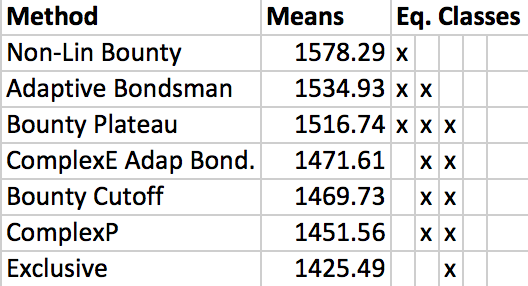
\includegraphics[width=3.3in]{staticT.png}\end{center}
\vspace{-0.5em}\caption{Experiment 1, A Static Environment, total time available metric.}
\label{staticT}
\end{figure}

\begin{figure}[t]
\begin{center}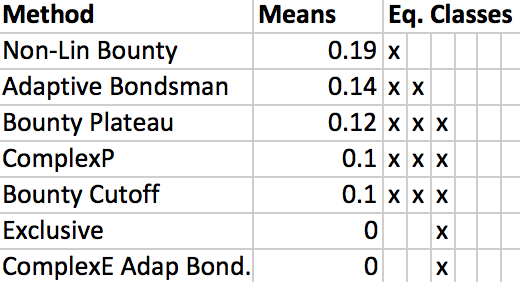
\includegraphics[width=3.3in]{staticR.png}\end{center}
\vspace{-0.5em}\caption{Experiment 1, A Static Environment, redundancy metric.}
\label{staticR}
\end{figure}

\subsection{Second Experiment: Dynamic Agents}

In the real world, agents are prone to failure. We tested each method's ability to adapt to a situation where agents were periodically removed from the game, then later reinstated.  In this experiment, agent 1 was removed every 30,000 timesteps, and agent 2 was removed every 60,000 timesteps.  Agents were reinserted 20,000 timesteps after removal.  Ideally while agents were gone,  teammates would adapt to cover for them.


\paragrapha{Results}

We discovered that all the methods would adapt quickly, as illustrated in Figure~\ref{disintegratingf}. The \textit{Complex} method converged to the {\it Greedy}  performance regardless of the number of agents in the game.  This is verified in Table~\ref{disintegrating}, which reflects the final timestep 200,000, when two agents were missing from the game.

We note in Figure~\ref{disintegratingf} that \textit{Complex} and \textit{ComplexR}  (shown Figure~\ref{disintegratingf}) had very high temporary peaks of poor performance compared to other methods whenever an agent would disappear: they had a larger state table and would be expected to take longer to adapt.   The 10\% random task exploration strategy once again did poorly compared to other methods. Note that \textit{Auction} outperformed  \textit{SimpleP} and \textit{SimpleR}, but not \textit{Complex}.



\begin{figure}[t]
\begin{center}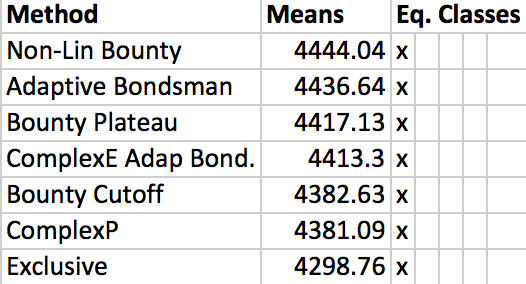
\includegraphics[width=3.3in]{dynAgentT.png}\end{center}
\vspace{-0.5em}\caption{Experiment 2, Dynamic Agents, total time available metric.}
\label{dynAgentT}
\end{figure}

\begin{figure}[t]
\begin{center}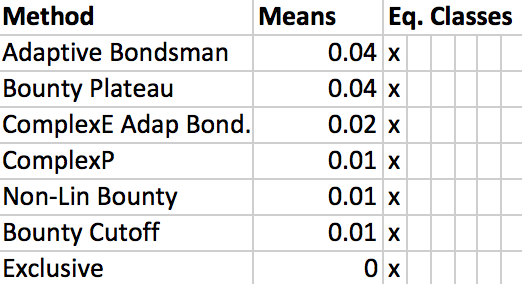
\includegraphics[width=3.3in]{dynAgentR.png}\end{center}
\vspace{-0.5em}\caption{Experiment 2, Dynamic Agents, redundancy metric.}
\label{dynAgentR}
\end{figure}



\subsection{Third Experiment: Dynamic Tasks}
If the distribution of tasks suddenly changes, we want the bounty system to recover.  To test this, we occasionally rotated the corners among the four agents: that is, agent~1's corner would become agent~2's corner, whose old corner would now belong to agent~3, and so on.  We did this every 25,000 timesteps, with a second rotation performed every 50,000 timesteps (a worst case scenario for task distribution, as the closest balls became the furthest and vice versa).

\paragrapha{Results}
This experiment, as shown in Figure~\ref{movingf} and Table~\ref{moving}, shows the weakness of relying solely on bounty for exploration: the \textit{Simple} and \textit{Complex} methods performed poorly.  Following them were the remaining random exploration methods (\textit{SimpleR}, and \textit{ComplexR}). Finally, the best adaptive methods were \textit{SimpleP}, \textit{Auction}, \textit{ComplexP}, and \textit{Exclusive}. We note that, \textit{SimpleP} and \textit{ComplexP}, performed just as well as the  \textit{Exclusive} and  \textit{Auction} methods. Unfortunately, no adaptive method could consistently converge to \textit{Greedy}'s performance.


%\bump

We also note that after several iterations of rotations, the agents were unable to converge to the same (lower) value.  This is because the rate of rotating was too fast for the adaptive methods to catch up and so the total bounty would gradually pile up. This was especially true for the \textit{Auction} strategy.  In the first few iterations \textit{Auctions} started out better than \textit{ComplexP}, but by the last iteration, they were equivalent.

\begin{figure}[t]
\begin{center}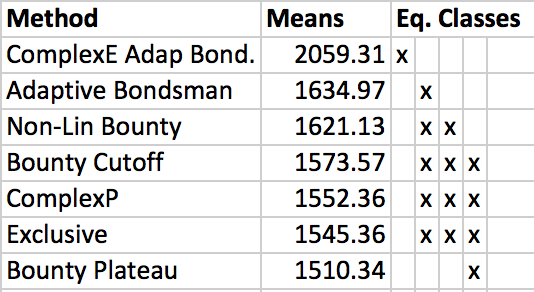
\includegraphics[width=3.3in]{rotT.png}\end{center}
\vspace{-0.5em}\caption{Experiment 3, Dynamic Tasks, total time available metric.}
\label{rotT}
\end{figure}

\begin{figure}[t]
\begin{center}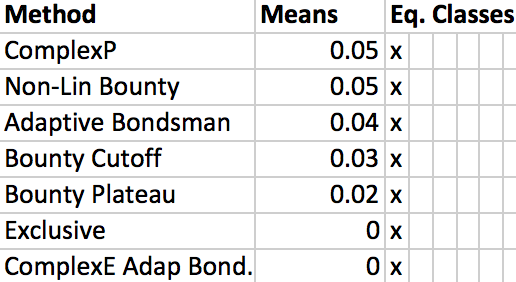
\includegraphics[width=3.3in]{rotR.png}\end{center}
\vspace{-0.5em}\caption{Experiment 3, Dynamic Tasks, redundancy metric.}
\label{rotR}
\end{figure}



\subsection{Fourth Experiment: Unreliable Collaborators}
The purpose of Experiments 4 and 5 is to show when exclusivity can fail. In the previous experiments exclusivity was favorable, since non-exclusive approaches potentially wasted time on tasks another agent was completing. However, in these next experiments we show there are situations where non-exclusivity is desirable.

Suppose a system has agents which do not perform nearly as well as other agents. In this experiment, there were 2 agents, placed in the top left corner of the grid world, who moved 10x slower than other agents, and 4 agents, placed in the corners (like normal), who moved at a normal speed. We chose to test \textit{ComplexP} as our main bounty mechanism, and compared it to our two auction-like algorithms (\textit{Auction} and \textit{Exclusive}).

\paragrapha{Results} The results are shown in Table~\ref{unreliableT} and illustrated in Figure~\ref{badrobotsf}.  \textit{ComplexP} was clearly the best in this test. The obvious underlying reason was that agents at normal speed would win a race to a ball (a task) against a slow, unreliable collaborator.  The auction-like methods simply had no way to prevent the unreliable collaborator from holding things up.  Also, \textit{ComplexP} was naturally suited to this task due to the added information it learned about the other agents in the environment.


\begin{figure}[t]
\begin{center}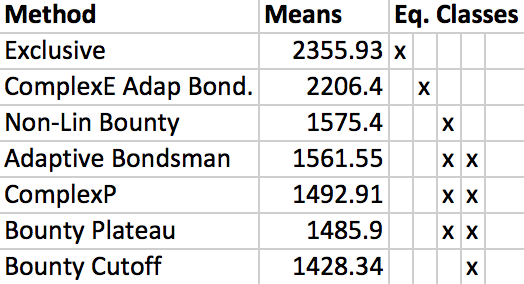
\includegraphics[width=3.3in]{badT.png}\end{center}
\vspace{-0.5em}\caption{Experiment 4, Unreliable Collaborators, total time available metric.}
\label{badT}
\end{figure}

\begin{figure}[t]
\begin{center}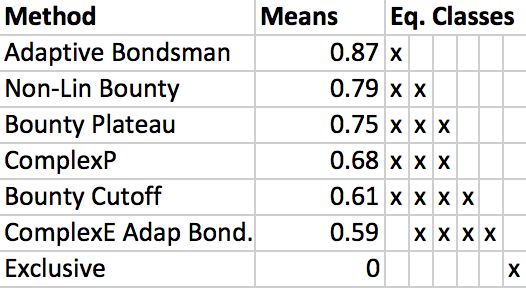
\includegraphics[width=3.3in]{badR.png}\end{center}
\vspace{-0.5em}\caption{Experiment 4, Unreliable Collaborators, redundancy metric.}
\label{badR}
\end{figure}



\subsection{Fifth Experiment: Unexpectedly Bad Tasks}
We now consider an experiment where some tasks suddenly change in difficulty for particular agents. We modified the scenario such that, every time a task class reappeared on the board, there was a 10\% probability it would become ``difficult'' for a randomly-selected agent to complete.  By ``difficult'' we mean that this agent, upon choosing this task, would move at 
one-tenth his normal speed. %If a task is already difficult for an agent to do, there is still a 1 in 10 chance it will become difficult for a different agent after reappearing. 

We once again compared \textit{ComplexP}, \textit{Exclusive}, and \textit{Auction}.
% in this experiment.

\paragrapha{Results} The results are shown in Table~\ref{trapT} and illustrated in Figure~\ref{badtasksf}.  \textit{ComplexP}, again, was the clear winner.  Once again, the exclusivity of the auction-like methods prevented agents from taking over ``difficult'' tasks which have trapped helpless agents.

\begin{figure}[t]
\begin{center}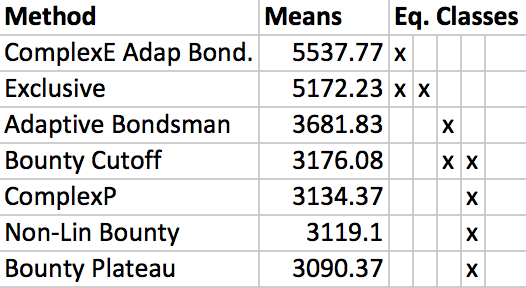
\includegraphics[width=3.3in]{trapsT.png}\end{center}
\vspace{-0.5em}\caption{Experiment 5, Unexpectedly Bad Tasks, total time available metric.}
\label{trapsT}
\end{figure}

\begin{figure}[t]
\begin{center}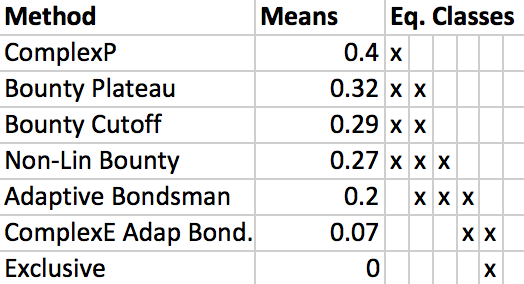
\includegraphics[width=3.3in]{trapsR.png}\end{center}
\vspace{-0.5em}\caption{Experiment 5, Unexpectedly Bad Tasks, redundancy metric.}
\label{trapsR}
\end{figure}


\vspace{-0.5em}
\section{Conclusions} 

We have demonstrated methods for agents to adapt to their best tasks in a bounty hunter system, thus improving the efficiency of the whole system.  We have compared various approaches to adaptation, as well as both exclusive and non-exclusive task allocation strategies.  

As we had imagined, the ``complex'' non-exclusive methods performed better in dynamic situations due to their additional per-agent information, since they retained knowledge of missing agents and could immediately re-use that information when the agents were re-introduced.    While the exclusive and ``auction-like'' methods generally performed well in the static and basic dynamic scenarios, Experiments 4 and 5 showed that they would perform very poorly in situations where task exclusivity could saddle agents with leaden tasks.  Without any additional information or communication, non-exclusive bounty agents naturally adapted to these situations. In the future, we will look at different scenarios which take advantage of this natural adaptation.  

A bounty hunter system is a promising method for task allocation: it seems robust to loss of agents, changes in task difficulty, and other kinds of noise.  The key properties of a bounty hunter system which distinguish it from other methods, and permits this robustness, is its non-exclusivity of task assignment, lack of a bidding structure, and the increasing attractiveness of outstanding tasks as the bounty on them rises.  For this reason, it is surprising bounties have not been studied more: we hope this trend will change in the future.


\vspace{-0.5em}
\bibliographystyle{plain}
\bibliography{bounty}


\end{document} 




